
Figure~\ref{fig:Drafting} shows the draft schedule establish \emph{a priori}

\begin{figure*}
% - Use the starred version in order to put floats on two columns
% - Possibly, use the "\ifscreen ... \else ... \fi"" alternative to orientate correctly
%   the planning with respect to the orientation of the paper (cf. below for the auto-evaluation)
   \centering
      
  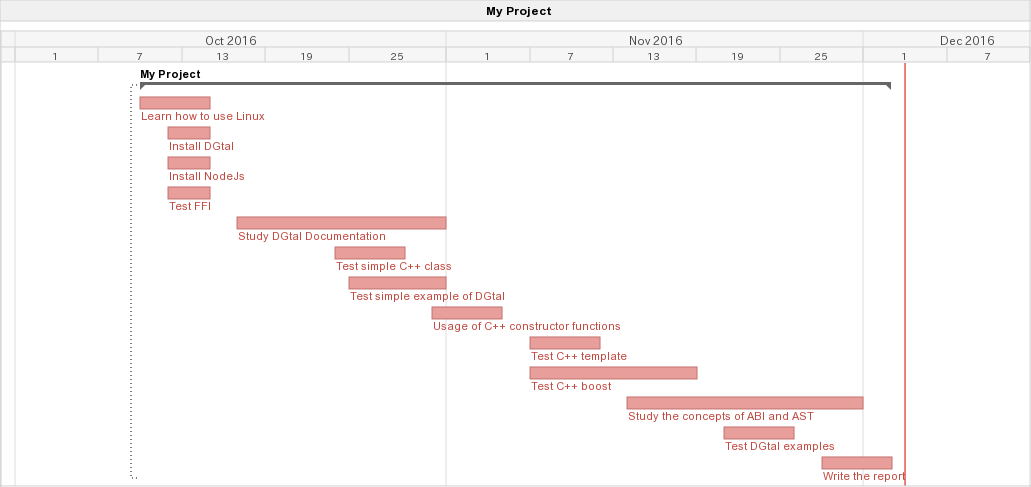
\includegraphics[scale=0.5]{Images/Gantt1.png}
  
   \caption{Drafting}
   \label{fig:Drafting}
\end{figure*}

Figure~\ref{fig:Planning} introduce the planning that has been build week after week during the course of the work.

\begin{figure*}
   \centering
      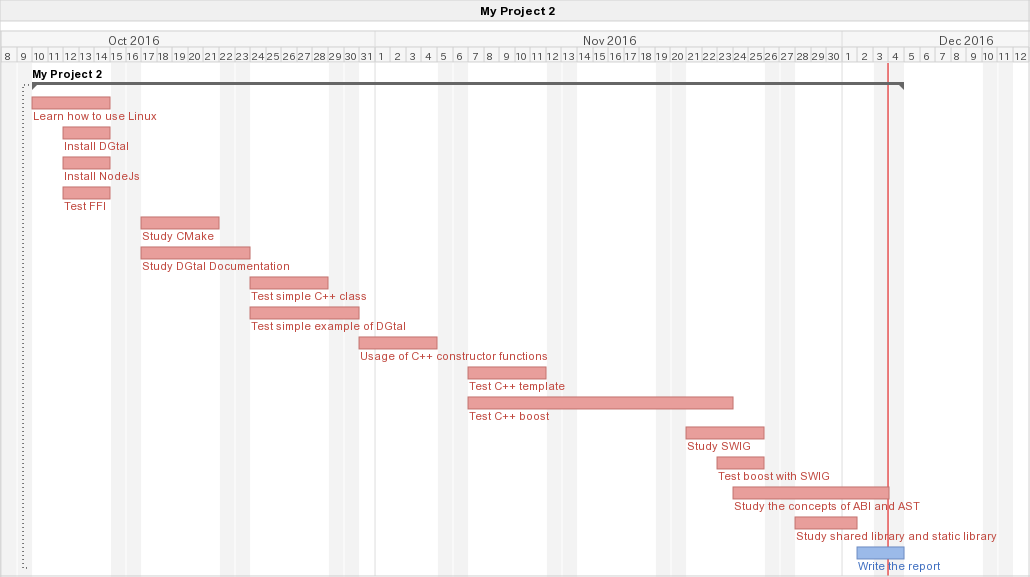
\includegraphics[scale=0.5]{Images/Gantt2.png}
   \caption{Planning}
   \label{fig:Planning}
\end{figure*}

There are two main difference of the drafting and the planning. We have planned to study the documentaion and test the examples of DGtal at very first time. However, the truth is we have under estimated of complexity of DGtal. The second difference is I've found the latest versions of SWIG can  warp c++ code for JavaScript, so I've spent quiet a lot of time to study it. 


\begin{comment}
Discuss differences between the drafting and the planning as well as lessons learned on the management of a research project or R\&D project.
\end{comment}
